\chapter{Ход работы}

\textbf{Цель работы}: провести модельное исследование импульсного понижающе-повышающего стабилизатора с использованием выбранных элементов.

Исходные данные: условия (дано) из ДЗ и результаты расчетов

\begin{figure}[h!]
	\centering
	\caption{Схема импульсного понижающе-повышающего стабилизатора}
	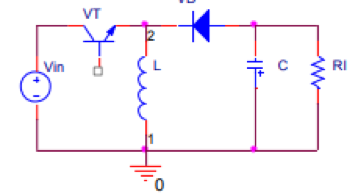
\includegraphics{images/1.png}
\end{figure}


\begin{figure}[h!]
	\centering
	\caption{Модель системы в OrCAD Capture}
	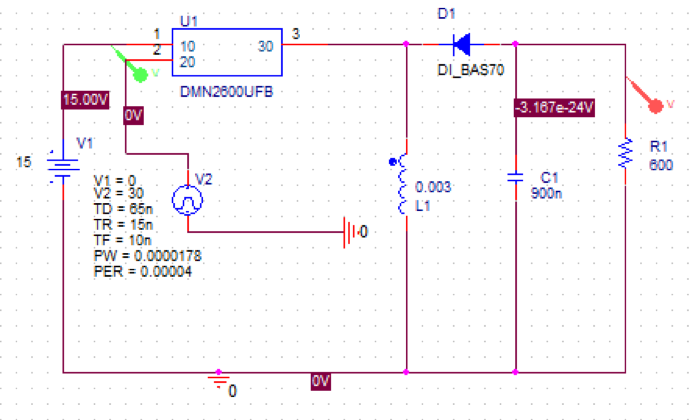
\includegraphics{images/2.png}
\end{figure}

\chapter{Результаты моделирования}

\begin{figure}[h!]
	\centering
	\caption{Выходное напряжение (зеленый, В), среднее выходное напряжение (красный, В)}
	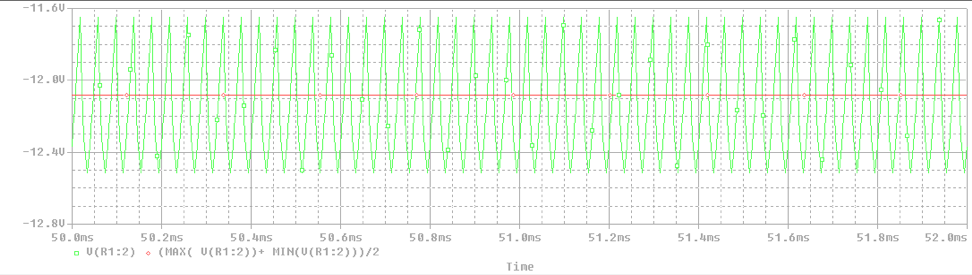
\includegraphics{images/3.png}
\end{figure}

\begin{figure}[h!]
	\centering
	\caption{Ток на дросселе (зеленый, А), средний ток на дросселе (красный, А)}
	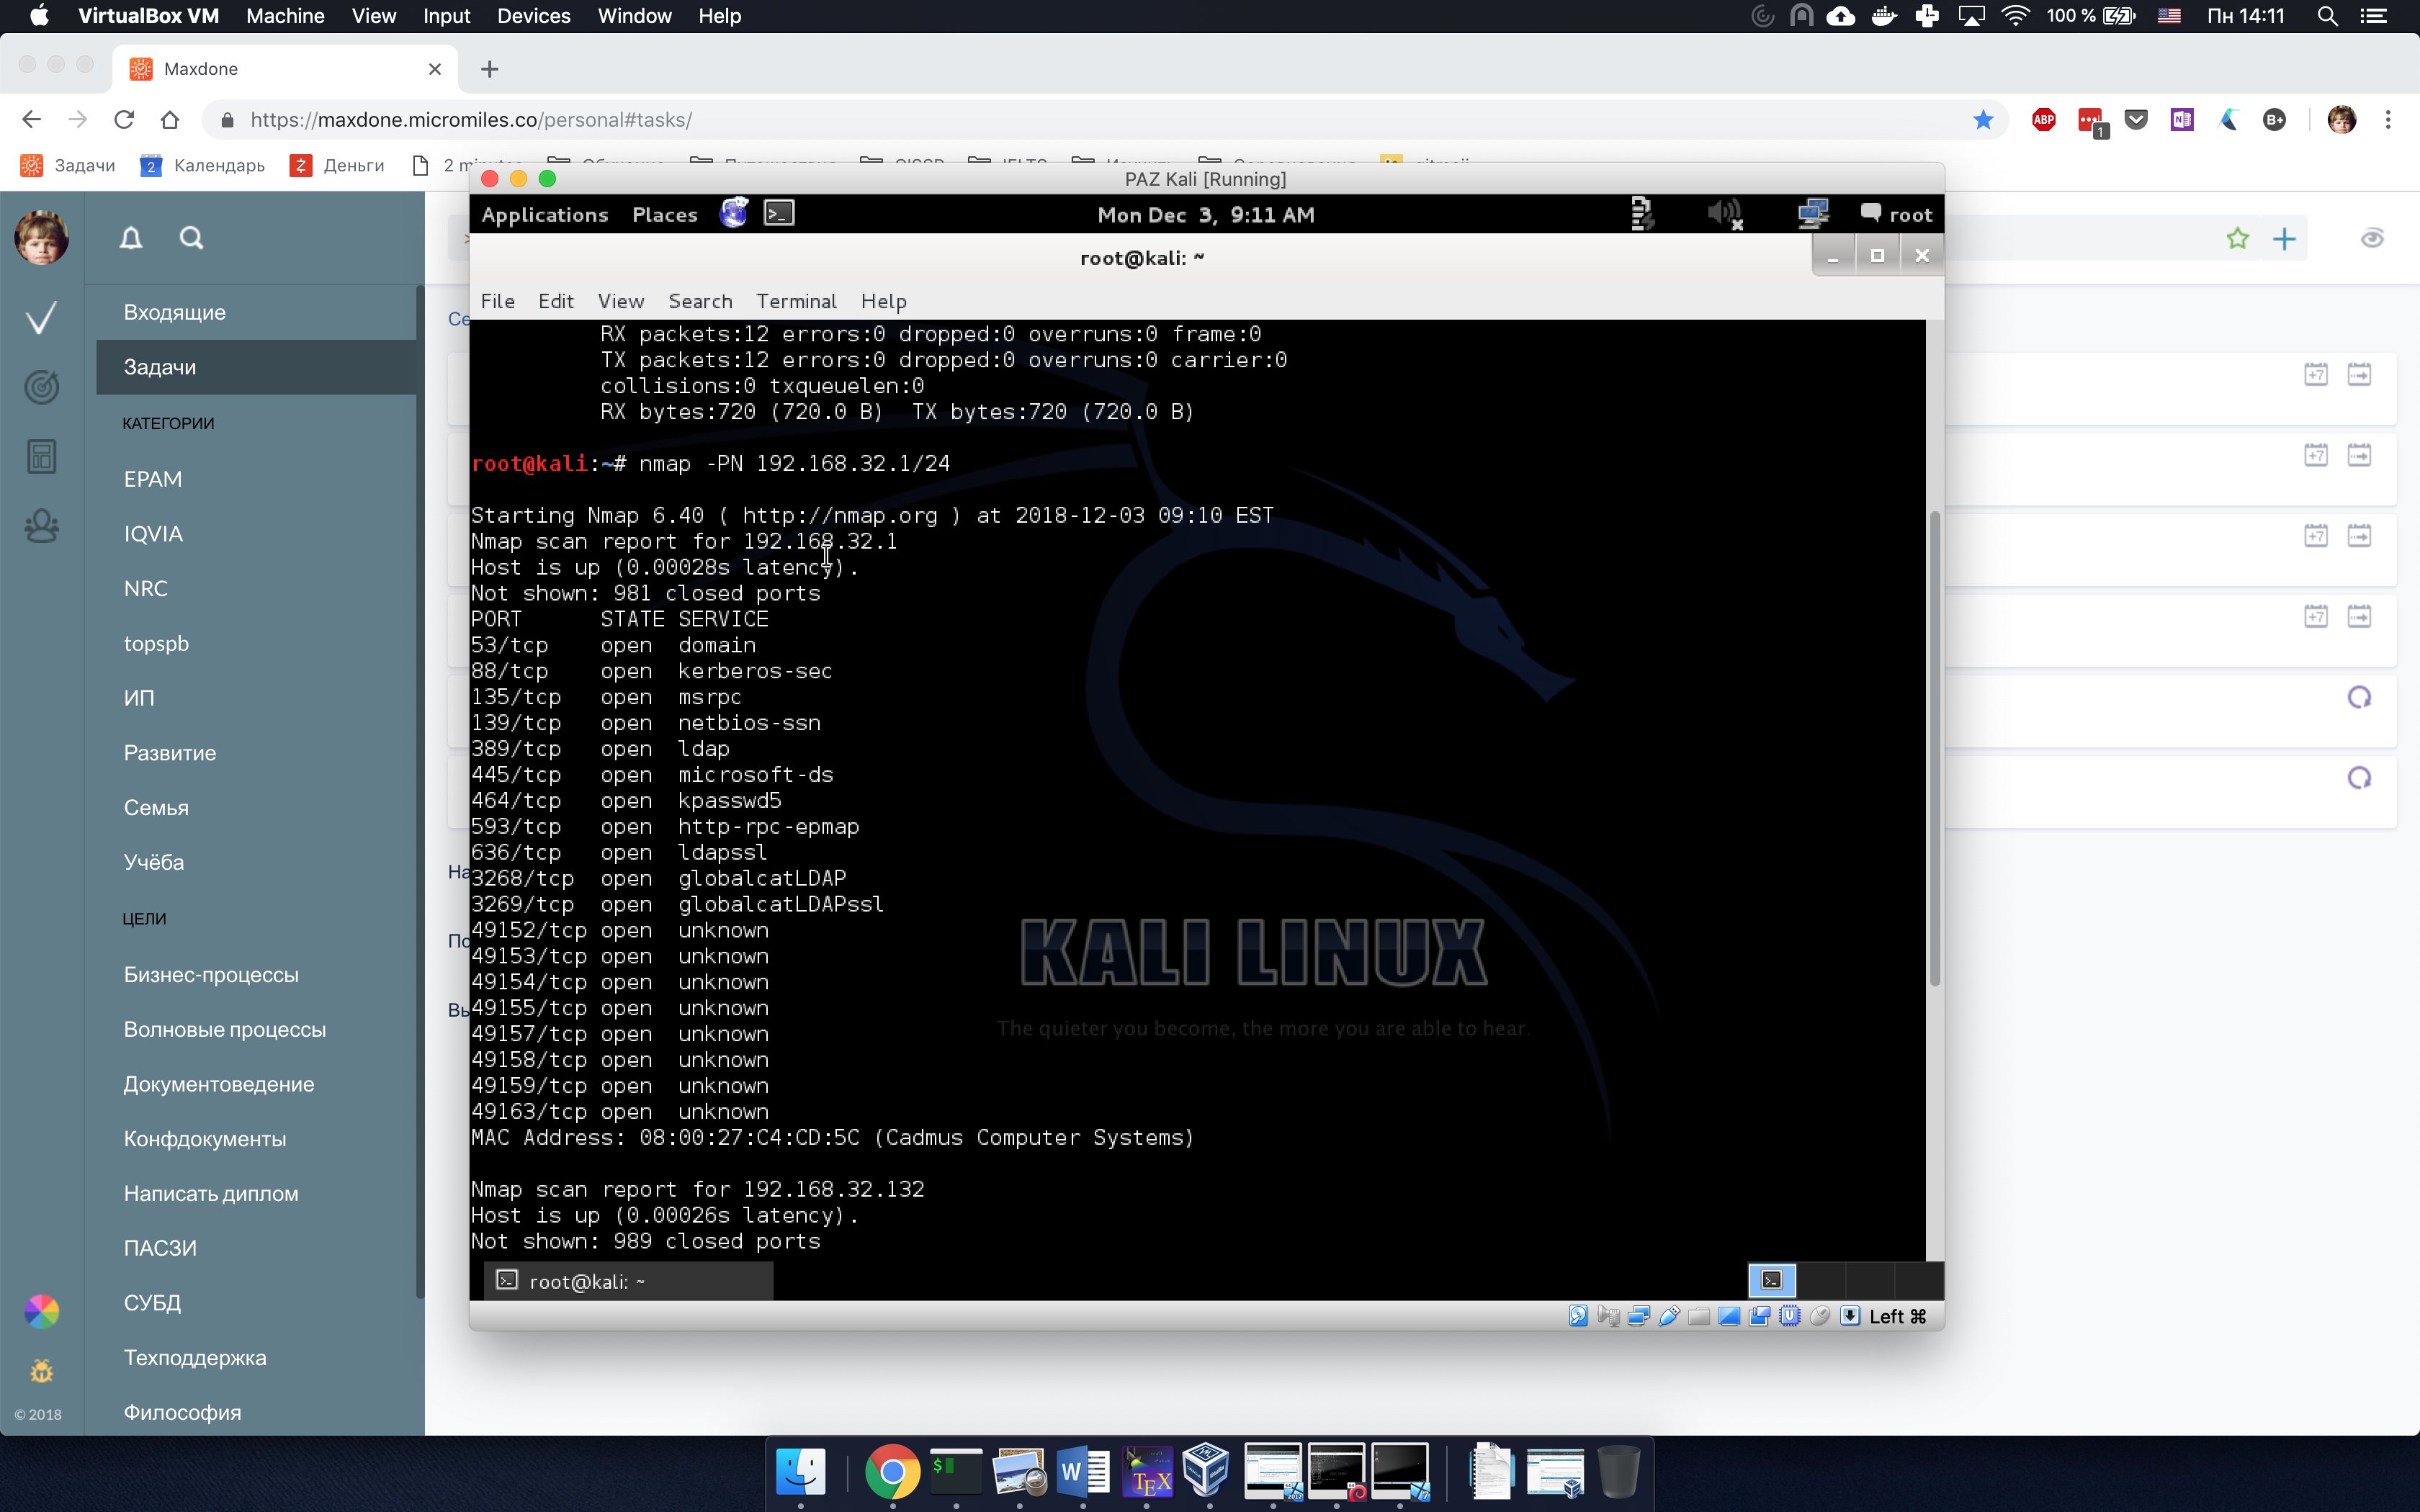
\includegraphics{images/4.png}
\end{figure}

\begin{figure}[h!]
	\centering
	\caption{Напряжение затвор-исток (зеленый, А), напряжение сток-исток (красный, А) }
	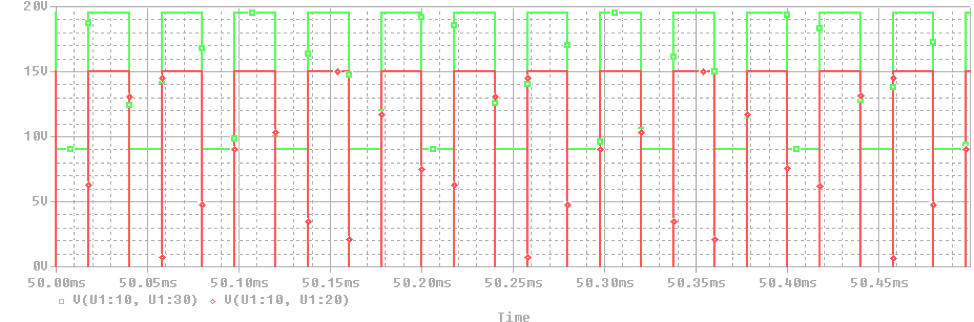
\includegraphics{images/5.png}
\end{figure}



\chapter{Измерения в OrCAD Capture}

Выходное напряжение, В:   				           

\[
U_{OUT\_AVG\_EXP}=-12.08
\]

Амплитуда пульсаций выходного напряжения, В:	
\[
\Delta U_{OUT\_EXP}=0.456
\]

Ток дросселя, А:	
		        				
\[
I_{L\_AVG\_EXP}=0.0385 
\]

Амплитуда пульсаций тока дросселя, А:			
\[
\Delta I_{L\_EXP}=0.456
\]


\section{Расчёт погрешностей}

Погрешность $U_{OUT}$:

\[
\left| \frac{U_{OUT\_EXP}-U_{OUT}}{U_{OUT}}\right|=0.7\%
\]


Погрешность $\Delta U_{OUT}$:

\[
\left| \frac{\Delta U_{OUT\_EXP}-\Delta U_{OUT}}{\Delta U_{OUT}}\right|=9 \%
\]

Погрешность $I_{L\_AVG}$:

\[
\left| \frac{I_{L\_AVG\_EXP}-I_{L\_AVG}}{I_{L\_AVG}} \right|=7 \%
\]

Погрешность $\Delta I_L$:

\[
\left| \frac{\Delta I_{L\_EXP}-\Delta I_L}{\Delta I_L}\right|=3 \%
\]

\chapter{Вывод}

В ходе выполнения лабораторной работы был промоделирован понижающе-повышающий стабилизатор, построены графики изменения величин в OrCAD PSpice, измерены необходимые величины по этим графикам и рассчитаны погрешности.

Ни одна из вычисленных погрешностей не превышает 10\%, что свидетельствует о корректности выполнения работы и соответствии модели расчетным значениям.


